% $Log: abstract.tex,v $
% Revision 1.1  93/05/14  14:56:25  starflt
% Initial revision
% 
% Revision 1.1  90/05/04  10:41:01  lwvanels
% Initial revision
% 
%
%% The text of your abstract and nothing else (other than comments) goes here.
%% It will be single-spaced and the rest of the text that is supposed to go on
%% the abstract page will be generated by the abstractpage environment.  This
%% file should be \input (not \include 'd) from cover.tex.
\begin{figure}[ht]
\centering
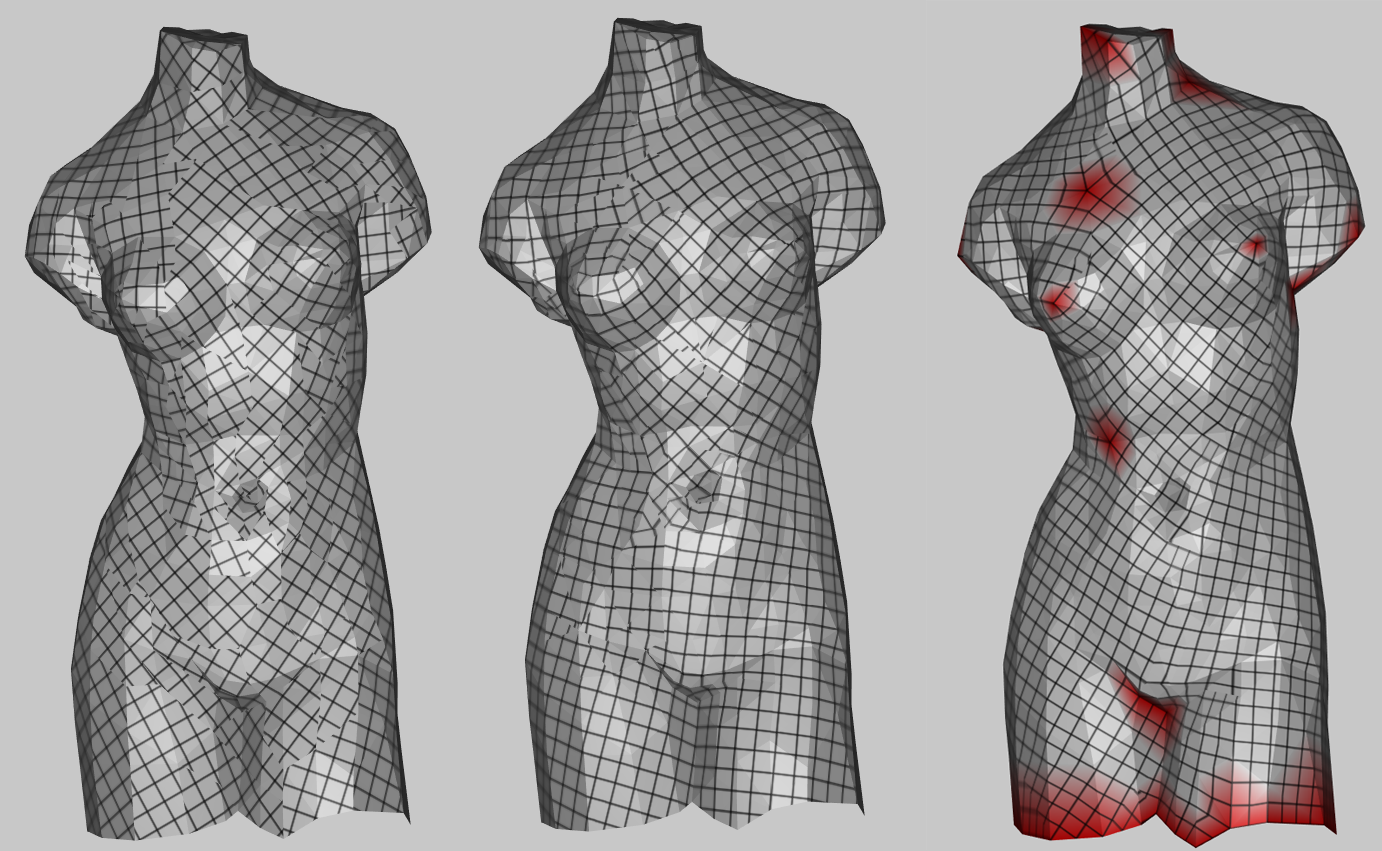
\includegraphics[width=15cm]{figures/teaser.png}
\caption[Abstract's Teaser]{\textbf{Left:} Initial mapping of cut mesh. \textbf{Middle:} With increased penalty on seamlessness violation. \textbf{Right:} With increased penalty on integer violation.}
\label{fig:teaser}
\end{figure}

\subsubsection{Introduction}
Many applications in computer graphics, such as character modeling and animation, architectural geometry, and also physical simulation to some extent, call for quad meshes as a representation of the geometry \cite{10.1111/cgf.12014}. However, since triangle meshes are generally more prevalent, they need to be convert via the process known as \emph{quad remeshing}.

\noindent Numerous techniques were introduced in recent years, and the most common approach is to split the problem into cross field generation, and field guided parameterization. In this document, we present an interactive, direct parametrization approach, which nullifies the need for intermediate steps.

\noindent The idea behind parameterization based methods in general, is to map the mesh to the plane, and create a regular grid layout on it. In order to ensure that the grid on the plane is transformed into a valid quad mesh on the surface, certain conditions on the parameterization must be fulfilled \cite{bommes:hal-00862648}:

\begin{enumerate}
  \item \textbf{Seamless Condition}: The transition function $g_{ij}$ between two half-edges $e_i$ and $e_j$ on the parameterization domain that corresponds to the same surface edge that is part of a cut seam, has to be an integer-grid automorphism given by:
  $$e_j = R^{r_{ij}}_{90^\circ}e_i + \vec{t}_{ij}$$
  Where  $r_{ij} \in \{0,1,2,3\}$ and $\vec{t}_{ij} \in \mathbb{Z}^2$.
  
  \item \textbf{Singular-Points Condition}: All singular vertices, which are characterized by a non-zero angular defect on the parameterization domain, have to lie on integer locations. That is, given the set $S_i$ of all parameterization domain vertices that correspond to the same singular surface vertex $v_i$, we require that:
  $$\forall u \in S_i: u \in \mathbb{Z}^2 $$
  
  \item \textbf{Consistent Orientation Condition}: All triangles on the parameterization domain should have the same orientation. That is, we should not allow triangle flips after initial mapping is formed.
\end{enumerate}

\subsubsection{Our Approach}
Inspired by \cite{Poranne:Autocuts:2017}, we employ a direct approach to the problem of quadrangulating a triangle mesh, by formulating and solving a smooth optimization problem. We model smooth penalty functions for the first two conditions mentioned above (Seamless and Singular-Points), and add to it an additional penalty, the Symmetric Dirichlet energy, which prevents triangle flips and penalize triangle distortion.
Since all of our penalty functions are smooth, we can analytically derive their gradients and hessians, and utilize Newton's method to iteratively solve for a mapping that renders a valid quad mesh on the 3D surface.

\noindent Our smooth approach allows us to visualize the whole optimization process for the end-user as an interactive design tool, which empowers the user to guide the algorithm to the desired result by gradually changing penalty weights, grid resolution, guiding quads direction using brush tool, and more. The user receives immediate feedback for any change applied to the problem settings. Figure \ref{fig:teaser} illustrates the three main stages of our approach. First, the 3D surface is cut into the plane. Then, the seamless penalty function weight gradually increased. Finally, the singular points penalty function is turned on to place singular vertices at integer locations.

\subsubsection{Details}
\paragraph{Initialization}
We cut the mesh by mapping its dual spanning tree to the parameterization plane isometrically as a triangle soup. We first map an arbitrary initial triangle to the parameterization plane. Then, we map to the plane all neighbour triangles of the initial triangle, such that adjacent triangles share an edge. We continue this process for the next layer of neighbours, till we map all of the mesh's triangles.
\subsubsection{Seamless Penalty Functions}
\paragraph{Angle Penalty}
Given two half-edges $e_i$ and $e_j$ on the parameterization domain that corresponds to the same surface edge, we penalize the angle between them as follows: 
$$P_{\mathrm{angle}}\left(e_i,e_j\right) = \sin\left(4\left(\theta(e_i) - \theta(e_j) \right) - \frac{\pi}{2} \right) + 1$$
Where $\theta(e_i)$ and $\theta(e_j)$ are the angles of the two half edges $e_i$ and $e_j$, respectively. For any $k \in \mathbb{Z}$ such that $\theta(e_i) - \theta(e_j) = \frac{\pi}{2}k$ we have that $P_{\mathrm{angle}}\left(e_i,e_j\right) = 0$. Therefore, $P_{\mathrm{angle}}$ will penalize half-edges of which their angle discrepancy differs from a multiple of $90^\circ$.
\paragraph{Length Penalty}
We penalize the length discrepancy between the two half-edges with the following penalty function:
$$P_{\mathrm{length}}\left(e_i,e_j\right) = \left( \norm{e_i}^2 - \norm{e_j}^2 \right)^2$$
Only when the two half-edges have the same length, we have that $P_{\mathrm{length}}\left(e_i,e_j\right) = 0$.
\paragraph{Translation Penalty}
We penalize for non-integer translation between the two half-edges as follows:
\begin{multline}
P_{\mathrm{translation}}\left(e_i,e_j\right) = \sin\left(2\pi\left(x_{e_i} - x_{e_j}\right) - \frac{\pi}{2} \right) + 1 \\ + \sin\left(2\pi\left(y_{e_i} - y_{e_j}\right) - \frac{\pi}{2} \right) + 1 \nonumber
\end{multline}
Where $\left(x_{e_i}, y_{e_i}\right)$ and $\left(x_{e_j}, y_{e_j}\right)$ are the coordinates of two corresponding vertices of the two half-edges $e_i$ and $e_j$.
\subsubsection{Singular-Points Penalty Function}
To satisfy the singularity points condition, all vertices on the parameterization domain which correspond to the same vertex on the surface, have to lie on integer locations if they are characterized by a non-zero angle defect in the domain. Therefore, we penalize singular points as follows:
\begin{multline}
P_{\mathrm{singularity}}\left(S\right) = \sum_{u \in S} \left( \sin\left(2 \pi x_{u} - \frac{\pi}{2} \right) + 1 + \sin\left(2 \pi y_{u} - \frac{\pi}{2} \right) + 1 \right) \nonumber
\end{multline}
Where $S$ is a set of domain vertices with non-zero angle defect, which correspond to the same surface vertex, and $\left(x_u,y_u\right)$ are the coordinates of the domain vertex $u \in S$. We weight $P_{\mathrm{singularity}}$ by the magnitude of the angle defect.
\subsubsection{Consistent Orientation and Distortion Penalty Functions}
To satisfy the consistent orientation condition, and to minimize triangle distortion, we use the symmetric dirichlet energy \cite{10.1145/2766947}, which prevents triangle flips. The symmetric dirichlet penalty function is given as follows:
$$
P_{\mathrm{dirichlet}}\left(t_i\right) = \norm{J\left(t_i\right)}_F^2 + \norm{J^{-1}\left(t_i\right)}_F^2 \nonumber
$$
Where $J\left(t_i\right)$ is the Jacobian of the mapping of triangle $t_i$ and $\norm{\cdot}_F$ is the Frobenius norm.
\subsubsection{Optimization Process}
In order to find a parameterization which forms a valid quad mesh on the 3D surface, we solve the following unconstrained optimization problem:
\begin{alignat}{2}
  &\min_{X}
     &\quad & \sum_{i \sim j} P_{\mathrm{angle}}\left(e_i,e_j\right) + P_{\mathrm{length}}\left(e_i,e_j\right) + P_{\mathrm{translation}}\left(e_i,e_j\right) \nonumber\\ 
  &  &  & + \sum_{i} P_{\mathrm{singularity}}\left(S_i\right) \nonumber\\ 
  &  &  & + \sum_{i} P_{\mathrm{dirichlet}}\left(t_i\right) \nonumber
\end{alignat}
Where $X$ denotes the set of variables of the optimization problem, i.e., the coordinates of the vertices in the parameterization domain. We derive the analytical expressions for the gradient and Hessian of each penalty function and make sure that all Hessians are positive semi-definite by zeroing negative eigenvalues. We solve the optimization problem using Newton's method. In iteration $n$, we evaluate the gradient $g^{(n)}$ and Hessian $H^{(n)}$ of our total objective function at $X^{(n)}$, and solve the Newton equation $H^{(n)}p^{(n)}=-g^{(n)}$ which yields a search direction $p^{(n)}$. The next iterate is obtained by $X^{(n+1)} = X^{(n)} + \alpha p^{(n)}$ where the optimal $\alpha$ is found using line search. We use Intel's Pardiso solver to solve the sparse Newton equation.
